% 
% (c) Copyright 2016 Tabea Mendez
% 
% This source is free: you can redistribute it and/or modify
% it under the terms of the GNU General Public License as published by
% the Free Software Foundation, either version 3 of the License, or
% (at your option) any later version.
% 
% This source is distributed in the hope that it will be useful,
% but WITHOUT ANY WARRANTY; without even the implied warranty of
% MERCHANTABILITY or FITNESS FOR A PARTICULAR PURPOSE.  See the
% GNU General Public License for more details.
% 
% You should have received a copy of the GNU General Public License
% along with this source.  If not, see <http://www.gnu.org/licenses/>.
%
%%%%%%%%%%%%%%%%%%%%%%%%%%%%%%%%%%%%%%%%%%%%%%%%%%%%%%%%%%%%%%%%%%%%%%%%%%%%%%

\section{Äquivalente Beschreibungen für digitale Filter}
	Um digitale Filter zu beschreiben, gibt es diverse Möglichkeiten.\\[0.2cm]
	\begin{minipage}{0.4\textwidth}
		\begin{itemize}
		 \item Übertragungsfunktion $H(z)$\\[-0.3cm]
		 \item Impulsantwort $h(n)$\\[-0.3cm]
		 \item Frequenzgang $H(\omega)$\\[-0.3cm]
		 \item I/O Differenzengleichung\\[-0.3cm]
		 \item Pol/Nullstellen-Diagramm\\[-0.3cm]
		 \item Realisation mit Blockdiagrammen\\ für Sampleverarbeitung\\[-0.3cm]
		 \item I/O Faltungsgleichungen für\\ Blockverarbeitung
		\end{itemize}
	\end{minipage}
	\begin{minipage}{0.6\textwidth}
		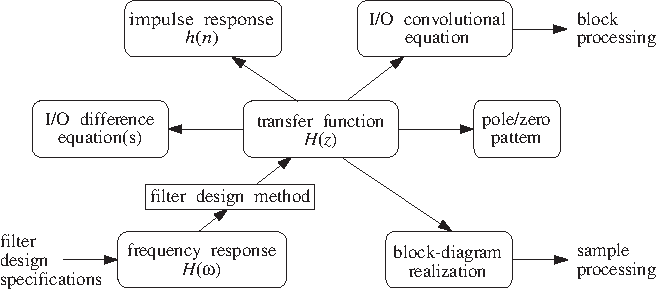
\includegraphics[width = 1\textwidth]{pic/transFunc.pdf}	
	\end{minipage}\\[0.3cm]

	\subsection{IIR und FIR Filter-Übertragungsfunktionen}
		\begin{itemize}
		 \item IIR Filter können im allgemeinen Fall als gebrochen rationale Funktionen dargestellt werden.\\[0.2cm]
		 \textbf{IIR}$\qquad$\fcolorbox{CadetRed}{white}{$H(z) = \dfrac{N(z)}{D(z)} = \dfrac{b_0 + b_1\,z^{-1} + b_2\,z^{-2} + \dots + b_N\,z^{-N} }{1 + a_1\,z^{-1} + a_2\,z^{-2} + \dots + a_M\,z^{-M} }$}
		 \item Das FIR Filter ist ein Spezialfall des IIR Filters ($a_i = 0$).\\[0.2cm]
		 \textbf{FIR}$\qquad$\fcolorbox{CadetRed}{white}{$H(z) = N(z) = b_0 + b_1\,z^{-1} + b_2\,z^{-2} + \dots + b_N\,z^{-N} $}
		\end{itemize}$ $\\[-0.8cm]

	\subsection{Impulsantwort \bm{$h(n)$}}
		\fcolorbox{CadetRed}{white}{$H(z)\quad \xrightarrow{\;\;Z^{-1}\;\;}\quad h(n)$}$\qquad\qquad$
		\fcolorbox{CadetRed}{white}{$h(n)\quad \xrightarrow{\;\;Z\;\;}\quad H(z)$}\\
		
	\subsection{I/O Differenzengleichung}
		$H(z)$ umformen, dass es bruchfrei und wird und $H(z)$ alleine auf der linken Seite steht.\\[0.2cm]
		$H(z)=\dfrac{N(z)}{D(z)}\qquad\Rightarrow\qquad H(z)\cdot \underbrace{\left[1 + a_1\,z^{-1}+ a_2\,z^{-2}+ ... + a_M\,z^{-M}\right]}_{D(z)}=\underbrace{\left[b_0 + b_1\,z^{-1}+ b_2\,z^{-2}+ ... + b_N\,z^{-N}\right]}_{N(z)}$\\[0.2cm]
		\begin{center}
			\fcolorbox{CadetRed}{white}{$H(z)= \underbrace{\left[b_0 + b_1\,z^{-1}+ b_2\,z^{-2}+ ... + b_N\,z^{-N}\right]}_{N(z)} - H(z)\cdot\underbrace{\left[a_1\,z^{-1}+ a_2\,z^{-2}+ ... + a_M\,z^{-M}\right]}_{D(z)-1}$}\\[0.2cm] $\text{\textcolor{white}{$Z$}}\;\text{\huge$\downarrow$}\;Z$\\[0.2cm]
			\fcolorbox{CadetRed}{white}{$h(n) = \left[b_0\,\delta(n) + b_1\,\delta(n-1)+ b_2\,\delta(n-2)+ ... + b_N\,\delta(n-N)\right] - \left[a_1\,h(n-1) + a_2\,h(n-2)+ ... + a_M\,h(n-M)\right]$}\\[0.2cm]
			$\delta(n) = x(n)\;\;\text{\huge$\downarrow$}\;\;h(n) = y(n)$\\[0.2cm]
			\fcolorbox{CadetRed}{white}{$y(n) = \left[b_0\,x(n) + b_1\,x(n-1)+ b_2\,x(n-2)+ ... + b_N\,x(n-N)\right] - \left[a_1\,y(n-1) + a_2\,y(n-2)+ ... + a_M\,y(n-M)\right]$}
		\end{center}$ $\\[-0.7cm]
\newpage
	\subsection{Frequenzgang \bm{$H(\omega)$}}
		In der Übertragungsfunktion $z$ durch $\e^{j\omega}$ ersetzen\\[0.2cm]
		\fcolorbox{CadetRed}{white}{$z = \e^{j\omega}$}$\qquad\rightarrow\qquad$
		\fcolorbox{CadetRed}{white}{$H(\omega) = H(z)|_{z = \e^{j\omega}} = \dfrac{b_0 + b_1\,\e^{-j\omega} + b_2\,\e^{-j\omega 2} + \dots + b_N\,\e^{-j\omega N} }{1 + a_1\,\e^{-j\omega} + a_2\,\e^{-j\omega 2} + \dots + a_M\,\e^{-j\omega M }}$}\\[0.2cm]
		Für den Betrag der Übertragungsfunktion $|H(\omega)|$ können Terme der Form $|1-a\,\e^{-j\omega}|$ noch vereinfacht werden.\\[0.2cm]
		\fcolorbox{CadetRed}{white}{$|1-a\,\e^{-j\omega}| = \sqrt{1-2a\cos(\omega)+a^2}$}\\[0.2cm]
		$|H(\omega)| = \dfrac{|1-z_1\,\e^{-j\omega}|\,|1-z_2\,\e^{-j\omega}|\,\dots\,|1-z_N\,\e^{-j\omega}|}{|1-p_1\,\e^{-j\omega}|\,|1-p_2\,\e^{-j\omega}|\,\dots\,|1-p_M\,\e^{-j\omega}|} = \dfrac{\sqrt{1-2z_1\cos(\omega)+z_1^2}\,\dots\,\sqrt{1-2z_N\cos(\omega)+z_N^2}}{\sqrt{1-2p_1\cos(\omega)+p_1^2}\,\dots\,\sqrt{1-2p_M\cos(\omega)+p_M^2}}$

	\subsection{Pol/Nullstellen - Diagramm}
		\begin{itemize}
		 \item Die Pole (Nullstellen von $D(z)$) und Nullstellen (Nullstellen von $N(z)$) können in der z-Ebene eingezeichnet werden.
		 \item Der Frequenzgang kann aus dem Pol/Nullstellen - Diagramm sehr einfach gezeichnet werden, indem ein man sich einen Punkt vorstellt, der von $0$ bis $\pi$ auf dem Einheitskreis wandert.
		 \subitem - Punkt fährt nahe am Pol vorbei $\quad\rightarrow\quad$ Frequenzgang wird gross.
		 \subitem - Punkt fährt nahe an Nullstelle vorbei $\quad\rightarrow\quad$ Frequenzgang wird klein.
		\end{itemize}
		\begin{minipage}{0.05\textwidth}$ $\end{minipage}
		\begin{minipage}{0.3\textwidth}
			\begin{tikzpicture}[>=latex', scale=1.4]
				\def\s{3};
				\def\f{1.3};
				\def\r{0.7};
				\def\a{60};
				\def\roc{0.9};

				\coordinate (c1) at (0,0);
	% 			\draw[line width=0.75,fill=CadetRed, opacity=0.5](c1)++(-\s/2,-\s/2)--++(\s,0)--++(0,\s)--++(-\s,0)--cycle ;
				\draw[line width=0.75](c1)++(-\s/2,-\s/2)node[above right]{kausal}--++(\s,0)--++(0,\s)node[below left]{$z$-Plane}--++(-\s,0)--cycle node[below right, CadetRed]{\textbf{ }};

	% 			\draw[line width=0.75,fill=white](c1)--++(-\f,0)--++(2*\f,0)--++(-\f,0)--++(0,-\f)--++(0,2*\f)--++(0,-\f)circle(\r);
				\draw[line width=0.75](c1)--++(-\f,0)--++(2*\f,0)--++(-\f,0)--++(0,-\f)--++(0,2*\f)--++(0,-\f)circle(0);

				\draw[line width=0.75,dashed](c1)--++(-\f,0)--++(2*\f,0)--++(-\f,0)--++(0,-\f)--++(0,2*\f)--++(0,-\f)circle(\roc);

				\draw[line width=0.75](c1)++(\roc,0.1)--++(0,-0.2)node[below right=-3pt,yshift=2pt]{1};


				\draw[line width=0.75,CadetRed,->](c1)++(0.4,0)arc(0:\a:0.4)node[yshift=-10pt,xshift=1pt]{\footnotesize$\omega$};

				\draw[line width=0.75,CadetRed,->](c1)--++({\roc*cos(\a)},{\roc*sin(\a)})--++({0.5*\roc*cos(90+\a)},{0.5*\roc*sin(90+\a)});
				\draw[line width=0.75,fill,CadetRed,->](c1)++({\roc*cos(\a)},{\roc*sin(\a)})circle(\r/15)node[above right=-1pt]{$\e^{j\omega}$};

				\draw[line width=0.75,fill,](c1)++(0.67,0.2)circle(\r/15)node[above left=-2pt,black]{$p_2$};
				\draw[line width=0.75,fill,](c1)++(0.67,-0.2)circle(\r/15)node[below left=-2pt,black]{$p_1$};
				\draw[line width=0.75,fill=white](c1)++(-\roc,0)circle(\r/15)node[above left=-1pt,black]{$z_1$};

				\draw[line width=0.75,fill=white](c1)++(-0.4,0.4)circle(\r/15)node[ right,black]{$z_2$};
				\draw[line width=0.75,fill=white](c1)++(-0.4,-0.4)circle(\r/15)node[right,black]{$z_3$};

			\end{tikzpicture}
		\end{minipage}
		\begin{minipage}{0.5\textwidth}
			\begin{tikzpicture}[>=latex', scale=1.4]
				\draw[->][line width=0.75](0,-0.2)--(0,2.8)node[right]{\footnotesize$|H(\omega)|$};
				\draw[->][line width=0.75](-0.2,0)--(3.6,0)node[below]{\footnotesize$\omega$};
				\draw[line width=0.75](-0,0.2)--(-0,-0.2)node[below]{$0$};
				\draw[line width=0.75](pi,0.2)--(pi,-0.2)node[below]{$\pi$};

				\draw[black, smooth,samples=100,domain=0:pi, line width=1,CadetRed]plot (\x,{0.12*(2.23607*sqrt(cos(\x*180/pi)+1)*sqrt(cos(\x*180/pi)+sin(\x*180/pi)+1.5)*sqrt(cos(\x*180/pi)-sin(\x*180/pi)+1.5))/(sqrt(-4*(cos(\x*180/pi)-0.25*sin(\x*180/pi)-0.25*4.2))*sqrt(-4*(4*cos(\x*180/pi)+sin(\x*180/pi)-4.2)))})node[above] {\footnotesize$ $};
			\end{tikzpicture}
		\end{minipage}

	\subsection{Realisation mit Blockdiagrammen}
		Es werden vier Arten von Blockdiagrammen unterschieden\\[0.2cm]
		\begin{minipage}{0.5\textwidth}
			\begin{itemize}
			\item Direktform (Siehe Seite 217)
			\item Parallelform (Siehe Seite 219)
			\end{itemize}
		\end{minipage}
		\begin{minipage}{0.5\textwidth}
			\begin{itemize}
			\item Kanonische Form (Siehe Seite 221)
			\item Transpolierte Form (Siehe Seite 222)
			\end{itemize}
		\end{minipage}$ $\\[-0.2cm]

		\textbf{Direktform}\\
		Aus der I/O Differenzengleichung kann direkt das Blockdiagramm der Direktform aufgezeichnet werden. Der Nachteil an dieser Variante ist, dass sehr viele Zustände gespeichert werden müssen.\\[0.2cm]
		\begin{tikzpicture}[>=latex', scale=1.1]
			\def\s{0.3};
			\def\l{1};
			\def\r{0.17};
			\def\dis{0.8};

			\coordinate (h1) at (0,0);
			\draw[line width=1,->](h1)++(0,-0.675)node[above right]{\footnotesize$x(n)$}--++(3.5-\r,0);
			\draw[line width=1,->](h1)++(3.5+\r,-0.675)--++(3.5-\r,0)node[above left]{\footnotesize$y(n)$};

			\foreach \i in {2,4,7}
			{
				\coordinate (h1) at (1,-\i/1.5);
				\draw[line width=1,fill=white](h1)++(-\s,-\s)--++(2*\s,0)--++(0,2*\s)--++(-2*\s,0)--cycle node at(h1)[xshift=0pt]{\footnotesize$z^{-1}$};
				\draw[line width=1,->](h1)++(0,0.675)--++(0,-0.38);
				\draw[line width=1,->](h1)++(0,-0.3)--++(0,-0.365)--++(2.5-\r,0);

				\coordinate (h1) at (6,-\i/1.5);
				\draw[line width=1,fill=white](h1)++(-\s,-\s)--++(2*\s,0)--++(0,2*\s)--++(-2*\s,0)--cycle node at(h1)[xshift=0pt]{\footnotesize$z^{-1}$};
				\draw[line width=1,->](h1)++(0,0.675)--++(0,-0.38);
				\draw[line width=1,->](h1)++(0,-0.3)--++(0,-0.365)--++(-2.5+\r,0);
			}

			\foreach \i in {2,4,6,9}
			{
				\coordinate (h1) at (2,{-(-1+\i)/1.5});
				\draw[line width=1,fill=white](h1)++(0,0)--++(0,1.2*\s)--++(2.2*\s,-1.2*\s)--++(-2.2*\s,-1.2*\s)--cycle;
			}

			\foreach \i in {4,6,9}
			{
				\coordinate (h1) at (5,{-(-1+\i)/1.5});
				\draw[line width=1,fill=white](h1)++(0,0)--++(0,1.2*\s)--++(-2.2*\s,-1.2*\s)--++(2.2*\s,-1.2*\s)--cycle;
			}

			\foreach \i in {2,4,6,9}
			{
				\coordinate (h1) at (3.5,{-(-1+\i)/1.5});
				\draw[line width=1,fill=white](h1)circle(\r)node{\Large$+$};
			}

			\foreach \i in {2,4,6,9}
			{
				\coordinate (h1) at (3.5,{-(-1+\i)/1.5});
				\draw[line width=1,fill=white](h1)circle(\r)node{\Large$+$};
			}
			\foreach \i in {4,6}
			{
				\coordinate (h1) at (3.5,{-(-1+\i)/1.5});
				\draw[line width=1](h1)++(0,\r)--++(0,0.5);
			}
			\coordinate (h1) at (3.5,{-(-1+9)/1.5});
			\draw[line width=1,->](h1)++(0,\r)--++(0,0.5)node[above=2pt]{$\vdots$};
			\foreach \i in {2,4,6}
			{
				\coordinate (h1) at (3.5,{-(-1+\i)/1.5});
				\draw[line width=1,->](h1)++(0,-0.5-\r)--++(0,0.5);
			}

			% x verzoegerungen
			\coordinate (h1) at (1,-4/1.5);
			\draw[line width=1](h1)++(0,0.675)node[left]{\footnotesize$x(n-1)$};
			\coordinate (h1) at (1,-6/1.5);
			\draw[line width=1,->](h1)++(0,0.675)node[left]{\footnotesize$x(n-2)$}--++(0,-0.3)node[yshift=-2.5pt]{$\vdots$};
			\coordinate (h1) at (1,-9/1.5);
			\draw[line width=1](h1)++(0,0.675)node[left]{\footnotesize$x(n-N)$};

			% y verzoegerungen
			\coordinate (h1) at (6,-4/1.5);
			\draw[line width=1](h1)++(0,0.675)node[right]{\footnotesize$y(n-1)$};
			\coordinate (h1) at (6,-6/1.5);
			\draw[line width=1,->](h1)++(0,0.675)node[right]{\footnotesize$y(n-2)$}--++(0,-0.3)node[yshift=-2.5pt]{$\vdots$};
			\coordinate (h1) at (6,-9/1.5);
			\draw[line width=1](h1)++(0,0.675)node[right]{\footnotesize$y(n-M)$};

			% B-Koeffizienten
			\coordinate (h1) at (2,{-(-1+2)/1.5});
			\draw[line width=1,fill=white](h1)node[right=-1pt]{\footnotesize$b_0$};
			\coordinate (h1) at (2,{-(-1+4)/1.5});
			\draw[line width=1,fill=white](h1)node[right=-1pt]{\footnotesize$b_1$};
			\coordinate (h1) at (2,{-(-1+6)/1.5});
			\draw[line width=1,fill=white](h1)node[right=-1pt]{\footnotesize$b_2$};
			\coordinate (h1) at (2,{-(-1+9)/1.5});
			\draw[line width=1,fill=white](h1)node[right=-1pt]{\footnotesize$b_N$};

			% A-Koeffizienten
			\coordinate (h1) at (5,{-(-1+4)/1.5});
			\draw[line width=1,fill=white](h1)node[left=-3pt]{\footnotesize-$a_1$};
			\coordinate (h1) at (5,{-(-1+6)/1.5});
			\draw[line width=1,fill=white](h1)node[left=-3pt]{\footnotesize-$a_2$};
			\coordinate (h1) at (5,{-(-1+9)/1.5});
			\draw[line width=1,fill=white](h1)node[left=-4pt]{\footnotesize-$a_M$};

		\end{tikzpicture}
		
		\textbf{Kanonische Form}\\
		Die Kanonische Form kann aus der Direktform abgeleitet werden. Dazu muss die rechte und linke Seite des Blockdiagrammes getauscht werden. Der Vorteil an dieser Variante ist, dass viel weniger Zustände gespeichert werden müssen.\\[0.2cm]
		\begin{tikzpicture}[>=latex', scale=1.1]
			\def\s{0.3};
			\def\l{1};
			\def\r{0.17};
			\def\dis{0.8};

			\coordinate (h1) at (0,0);
			\draw[line width=1,->](h1)++(0,-0.675)node[above right]{\footnotesize$x(n)$}--++(1-\r,0);
			\draw[line width=1,->](h1)++(1+\r,-0.675)--++(5-2*\r,0);
			\draw[line width=1,->](h1)++(3.5+\r,-0.675)--++(3.5-\r,0)node[above left]{\footnotesize$y(n)$};
			
			%verzoegerer
			\foreach \i in {2,4}
			{
				\coordinate (h1) at (3.5,-\i/1.5);
				\draw[line width=1,fill=white](h1)++(-\s,-\s)--++(2*\s,0)--++(0,2*\s)--++(-2*\s,0)--cycle node at(h1)[xshift=0pt]{\footnotesize$z^{-1}$};
				\draw[line width=1,->](h1)++(0,0.675)--++(0,-0.38);
				\draw[line width=1,->](h1)++(0,-0.3)--++(0,-0.365)--++(2.5-\r,0);
				\draw[line width=1,->](h1)++(0,-0.3)--++(0,-0.365)--++(-2.5+\r,0);
			}
			\coordinate (h1) at (3.5,-7/1.5);
			\draw[line width=1,fill=white](h1)++(-\s,-\s)--++(2*\s,0)--++(0,2*\s)--++(-2*\s,0)--cycle node at(h1)[xshift=0pt]{\footnotesize$z^{-1}$};
			\draw[line width=1,->](h1)++(0,0.675)--++(0,-0.38);
			\draw[line width=1](h1)++(0,-0.3)--++(0,-0.365)--++(2.5,0)--++(0,0.5);
			\draw[line width=1](h1)++(0,-0.3)--++(0,-0.365)--++(-2.5,0)--++(0,0.5);


		% 	% verstaerker rechts
			\foreach \i in {2,4,6,9}
			{
				\coordinate (h1) at (4.75,{-(-1+\i)/1.5});
				\draw[line width=1,fill=white](h1)++(0,0)--++(0,1.2*\s)--++(2.2*\s,-1.2*\s)--++(-2.2*\s,-1.2*\s)--cycle;
			}

			% verstaerker links
			\foreach \i in {4,6,9}
			{
				\coordinate (h1) at (2.25,{-(-1+\i)/1.5});
				\draw[line width=1,fill=white](h1)++(0,0)--++(0,1.2*\s)--++(-2.2*\s,-1.2*\s)--++(2.2*\s,-1.2*\s)--cycle;

			}

			% Addierer rechts
			\foreach \i in {2,4,6}
			{
				\coordinate (h1) at (6,{-(-1+\i)/1.5});
				\draw[line width=1,fill=white](h1)circle(\r)node{\Large$+$};
			}
			\foreach \i in {4,6}
			{
				\coordinate (h1) at (6,{-(-1+\i)/1.5});
				\draw[line width=1](h1)++(0,\r)--++(0,0.5);
			}
			\coordinate (h1) at (6,{-(-1+9)/1.5});
			\draw[line width=1,->](h1)++(0,\r)--++(0,0.5)node[above=2pt]{$\vdots$};
			\foreach \i in {2,4,6}
			{
				\coordinate (h1) at (6,{-(-1+\i)/1.5});
				\draw[line width=1,->](h1)++(0,-0.5-\r)--++(0,0.5);
			}
			% Addierer links
			\foreach \i in {2,4,6}
			{
				\coordinate (h1) at (1,{-(-1+\i)/1.5});
				\draw[line width=1,fill=white](h1)circle(\r)node{\Large$+$};
			}
			\foreach \i in {4,6}
			{
				\coordinate (h1) at (1,{-(-1+\i)/1.5});
				\draw[line width=1](h1)++(0,\r)--++(0,0.5);
			}
			\coordinate (h1) at (1,{-(-1+9)/1.5});
			\draw[line width=1,->](h1)++(0,\r)--++(0,0.5)node[above=2pt]{$\vdots$};
			\foreach \i in {2,4,6}
			{
				\coordinate (h1) at (1,{-(-1+\i)/1.5});
				\draw[line width=1,->](h1)++(0,-0.5-\r)--++(0,0.5);
			}

			% x verzoegerungen
			\coordinate (h1) at (3.5,-4/1.5);
			\draw[line width=1](h1)++(0,0.675)node[above left=-3pt]{\footnotesize$w(n-1)$};
			\coordinate (h1) at (3.5,-6/1.5);
			\draw[line width=1,->](h1)++(0,0.675)node[above left=-3pt]{\footnotesize$w(n-2)$}--++(0,-0.3)node[yshift=-2.5pt]{$\vdots$};

			% B-Koeffizienten
			\coordinate (h1) at (4.75,{-(-1+2)/1.5});
			\draw[line width=1,fill=white](h1)node[right=-1pt]{\footnotesize$b_0$};
			\coordinate (h1) at (4.75,{-(-1+4)/1.5});
			\draw[line width=1,fill=white](h1)node[right=-1pt]{\footnotesize$b_1$};
			\coordinate (h1) at (4.75,{-(-1+6)/1.5});
			\draw[line width=1,fill=white](h1)node[right=-1pt]{\footnotesize$b_2$};
			\coordinate (h1) at (4.75,{-(-1+9)/1.5});
			\draw[line width=1,fill=white](h1)node[right=-1pt]{\footnotesize$b_N$};

			% A-Koeffizienten
			\coordinate (h1) at (2.25,{-(-1+4)/1.5});
			\draw[line width=1,fill=white](h1)node[left=-3pt]{\footnotesize-$a_1$};
			\coordinate (h1) at (2.25,{-(-1+6)/1.5});
			\draw[line width=1,fill=white](h1)node[left=-3pt]{\footnotesize-$a_2$};
			\coordinate (h1) at (2.25,{-(-1+9)/1.5});
			\draw[line width=1,fill=white](h1)node[left=-4pt]{\footnotesize-$a_M$};

		\end{tikzpicture}

		\textbf{Transpolierte Form}\\
		Die Transpolierte Form kann aus der Kanonischen Form abgeleitet werden. Dazu muss das Blockdiagramm transponiert werden, d.h. Addierer mit Knoten und Knoten mit Addierer ersetzen, alle Flussrichtungen umkehren und Ein- und Ausgang vertauschen.\\[0.2cm]
		\begin{tikzpicture}[>=latex', scale=1.1]
			\def\s{0.3};
			\def\l{1};
			\def\r{0.17};
			\def\dis{0.8};

			\coordinate (h1) at (0,0);
			\draw[line width=1,->](h1)++(0,-0.675)node[above right]{\footnotesize$x(n)$}--++(3.5-\r,0);
			\draw[line width=1,->](h1)++(3.5+\r,-0.675)--++(3.5-\r,0)node[above left]{\footnotesize$y(n)$};

			\foreach \i in {2,4,7}
			{
				\coordinate (h1) at (1,-\i/1.5);
				\draw[line width=1,->](h1)++(0,0.65)--++(0,-1.315)--++(2.5-\r,0);

				\coordinate (h1) at (6,-\i/1.5);
				\draw[line width=1,->](h1)++(0,0.65)--++(0,-1.315)--++(-2.5+\r,0);
			}

			\foreach \i in {2,4,6,9}
			{
				\coordinate (h1) at (1.75,{-(-1+\i)/1.5});
				\draw[line width=1,fill=white](h1)++(0,0)--++(0,1.2*\s)--++(2.2*\s,-1.2*\s)--++(-2.2*\s,-1.2*\s)--cycle;
			}

			\foreach \i in {4,6,9}
			{
				\coordinate (h1) at (5.25,{-(-1+\i)/1.5});
				\draw[line width=1,fill=white](h1)++(0,0)--++(0,1.2*\s)--++(-2.2*\s,-1.2*\s)--++(2.2*\s,-1.2*\s)--cycle;
			}

			\foreach \i in {2,4,6,9}
			{
				\coordinate (h1) at (3.5,{-(-1+\i)/1.5});
				\draw[line width=1,fill=white](h1)circle(\r)node{\Large$+$};
			}

			\foreach \i in {2,4,6,9}
			{
				\coordinate (h1) at (3.5,{-(-1+\i)/1.5});
				\draw[line width=1,fill=white](h1)circle(\r)node{\Large$+$};
			}
			\foreach \i in {4,6}
			{
				\coordinate (h1) at (3.5,{-(-1+\i)/1.5});
				\draw[line width=1](h1)++(0,\r)--++(0,0.5);
			}
			\coordinate (h1) at (3.5,{-(-1+9)/1.5});
			\draw[line width=1,->](h1)++(0,\r)--++(0,0.5)node[above=2pt]{$\vdots$};
			\foreach \i in {2,4,6}
			{
				\coordinate (h1) at (3.5,{-(-1+\i)/1.5});
				\draw[line width=1,->](h1)++(0,-0.5-\r)--++(0,0.5);
			}

			\foreach \i in {2,4}
			{
				\coordinate (h1) at (3.5,-\i/1.5-0.1);
				\draw[line width=1,fill=white](h1)++(-\s,-\s)--++(2*\s,0)--++(0,2*\s)--++(-2*\s,0)--cycle node at(h1)[xshift=0pt]{\footnotesize$z^{-1}$};
			}

			\coordinate (h1) at (6,-6/1.5);
			\draw[line width=1,->](h1)++(0,0.675)--++(0,-0.3)node[yshift=-3pt]{$\vdots$};
			\coordinate (h1) at (1,-6/1.5);
			\draw[line width=1,->](h1)++(0,0.675)--++(0,-0.3)node[yshift=-3pt]{$\vdots$}; 


			% verzoegerungen
			\coordinate (h1) at (3.5,-4/1.5);
			\draw[line width=1](h1)++(0,0.675)node[right, yshift=33pt]{\footnotesize$w(n-1)$};
			\coordinate (h1) at (3.5,-6/1.5);
			\draw[line width=1](h1)++(0,0.675)node[right, yshift=33pt]{\footnotesize$w(n-2)$};

			% B-Koeffizienten
			\coordinate (h1) at (1.75,{-(-1+2)/1.5});
			\draw[line width=1,fill=white](h1)node[right=-1pt]{\footnotesize$b_0$};
			\coordinate (h1) at (1.75,{-(-1+4)/1.5});
			\draw[line width=1,fill=white](h1)node[right=-1pt]{\footnotesize$b_1$};
			\coordinate (h1) at (1.75,{-(-1+6)/1.5});
			\draw[line width=1,fill=white](h1)node[right=-1pt]{\footnotesize$b_2$};
			\coordinate (h1) at (1.75,{-(-1+9)/1.5});
			\draw[line width=1,fill=white](h1)node[right=-1pt]{\footnotesize$b_N$};

			% A-Koeffizienten
			\coordinate (h1) at (5.25,{-(-1+4)/1.5});
			\draw[line width=1,fill=white](h1)node[left=-3pt]{\footnotesize-$a_1$};
			\coordinate (h1) at (5.25,{-(-1+6)/1.5});
			\draw[line width=1,fill=white](h1)node[left=-3pt]{\footnotesize-$a_2$};
			\coordinate (h1) at (5.25,{-(-1+9)/1.5});
			\draw[line width=1,fill=white](h1)node[left=-4pt]{\footnotesize-$a_M$};
		\end{tikzpicture}
		
\section{Systemantwort auf sinusförmiges Eingangssignal}
	Wenn in ein LTI-System ein sinusförmiges Eingangssignal gegeben wird, so wird auch ein sinusförmiges Ausgangssignal derselben Frequenz herauskommen.\\[0.2cm]
	\begin{minipage}{0.5\textwidth}
		\begin{tikzpicture}[>=latex', scale=1]
			\draw[<-,line width=1](-0.6,0)--(-3.2,0)node[above right]{$x(n)=\e^{j\omega_0n}$};
			\draw[->,line width=1](0.6,0)--(4.2,0)node[above left]{$y(n) = H(\omega_0)\,\e^{j\omega_0n}$};
			\draw[line width=1](-0.6,-0.6)--(-0.6,0.6)--node [above]{LTI}(0.6,0.6)--(0.6,-0.6)--(-0.6,-0.6)node at (0,0){$H$};
		\end{tikzpicture} 
	\end{minipage}
	\begin{minipage}{0.5\textwidth}
		\fcolorbox{CadetRed}{white}{$\begin{array}{lcl}\e^{j\omega_0n}&\quad\xrightarrow{\;\;H\;\;} &\quad H(\omega_0)\,\e^{j\omega_0n}\\\e^{j\omega_0n}&\quad\xrightarrow{\;\;H\;\;} &\quad |H(\omega_0)|\,\e^{j\omega_0n + jarg(H(\omega_0))} \end{array}\\  $}
	\end{minipage}\\[0.2cm]

	\begin{minipage}{0.55\textwidth}
	Ein LTI System:\\[-0.35cm]
		\begin{itemize}
		\item erzeugt keine neuen Frequenzen\\[-0.35cm]
		\item dämpft/verstärkt das Signal mit $|H(\omega_0)|$\\[-0.35cm]
		\item verzöger das Signal um $arg(H(\omega_0))$\\[-0.35cm]
		\item erscheint am Ausgang mit derselben Frequenz\\[0.2cm]
		\end{itemize}

		\fcolorbox{CadetRed}{white}{$\begin{array}{lcl}\cos(\omega_0n)&\quad\xrightarrow{\;\;H\;\;} &\quad |H(\omega_0)|\cdot\cos(\omega_0n + arg(H(\omega_0)))\\\sin(\omega_0n)&\quad\xrightarrow{\;\;H\;\;} &\quad |H(\omega_0)|\cdot\sin(\omega_0n + arg(H(\omega_0))) \end{array}\\  $}
	\end{minipage}
	\begin{minipage}{0.45\textwidth}
		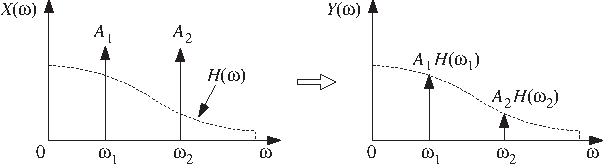
\includegraphics[width = 1\textwidth]{pic/frequenzgang.pdf}\\[1cm]
	\end{minipage}
\newpage
	\subsection{Phasen- und Gruppenverzögerung}
		\textbf{Phasenverzögerung}\\[0.1cm]
		Die Phasenverzögerung beschreibt, welche Frequenz um wie viele Samples verzögert wird. Die Anzahl verzögerter Samples muss nicht ganzzahlig sein.\\[0.2cm]
		\fcolorbox{CadetRed}{white}{$d(\omega) = -\dfrac{arg(H(\omega))}{\omega}$}$\qquad\rightarrow\quad \e^{j\omega n} \;\xrightarrow{\;H\;} \;|H(\omega)|\,\e^{j\omega (n-d(\omega))}$\\[0.3cm]
		Verzögert das Filter alle Frequenzen um die selbe Anzahl Samples, handelt es sich um ein linearphasiges Filter\\[0.2cm]
		\fcolorbox{CadetRed}{white}{$\text{linearphasiges Filter}\quad\Leftrightarrow\quad d(\omega) = D = \text{konstant}$}\\[0.2cm]
		$\rightarrow$ FIR Filter können sehr einfach als linearphasige Filter designed werden.\\[0.2cm]
		\textbf{Gruppenverzögerung}\\[0.2cm]
		\begin{minipage}{0.25\textwidth}
			\fcolorbox{CadetRed}{white}{$d_g(\omega) = -\dfrac{d\,arg(H(\omega))}{d\omega}$}
		\end{minipage}
		\begin{minipage}{0.75\textwidth}
			Wenn in einem Frequenzintervall alle Frequenzen dieselbe Phasenverzögerung haben, ist die Gruppenverzögerung eine Konstante.
		\end{minipage}

	\subsection{Einschwingvorgang}
		Wird eine Schwinung eingeschaltet, so braucht das Filter eine gewisse Zeit, bis es eingeschwungen ist\\ (im steady state).\\[0.2cm]
		\begin{tabularx}{0.9\textwidth}{p{3.1cm}cl}
			\textbf{Einschaltsignal:} && $x(n) = \e^{j\omega_0n}\,u(n)$\\[0.2cm]
			&& $X(z)=\dfrac{1}{1-\e^{j\omega_0}\,z^{-1}}\quad\qquad \text{ROC }|z|>1$\\[0.5cm]
		 \hline&&\\[-0.2cm]
			\textbf{Filter:} && $H(z)=\dfrac{N(z)}{D(z)} = \dfrac{N(z)}{(1-p_1\,z^{-1})\,(1-p_1\,z^{-1})\,\dots\,(1-p_M\,z^{-1})}$\\[0.5cm]
		\hline&&\\[-0.2cm]
			\textbf{Ausgangssignal:} && $Y(Z) = \dfrac{H(\omega_0)}{1-\e^{j\omega_0}\,z^{-1}}+\dfrac{B_1}{1-p_1\,z^{-1}}+\dfrac{B_2}{1-p_2\,z^{-1}}+\dots+\dfrac{B_M}{1-p_M\,z^{-1}}$\\[0.5cm]
			&& \fcolorbox{CadetRed}{white}{$y(n) = H(\omega_0)\,\e^{j\omega_0n} + \underbrace{B_1\,p_1^n+B_2\,p_2^n+\dots+B_M\,p_M^n}_{\text{Einschwingvorgang}}$}\\[0.9cm]
		\hline&&\\[-0.2cm]
			\textbf{Übergang in\newline Steady State}&&\fcolorbox{CadetRed}{white}{Alle Pole $|p_i|<1\qquad\Rightarrow\qquad \mylim{n\to\infty}{y(n)} = H(\omega_0)\,\e^{j\omega_0n}$}\\
		\end{tabularx}\\[0.2cm] 

		\textbf{Einschwingzeit:}\\[0.2cm]
			Der Pol am nächsten beim Einheitskreis dominiert die Zeitdauer des Einschwingvorganges\\[0.2cm]
			\fcolorbox{CadetRed}{white}{$\rho = \max\limits_{i}^{}\left\{|p_i|\right\}$} \\[0.2cm]
			Der Steady State gilt als erreicht, wenn der Beitrag des langsamste Pols unter 1\% gefallen ist.\\[0.2cm]
			\fcolorbox{CadetRed}{white}{$\rho^{n_{\text{eff}}} = \epsilon = 0.01$}$\qquad\Rightarrow\qquad$\textbf{Zeitkonstante des Filters:}$\qquad$\fcolorbox{CadetRed}{white}{$n_{\text{eff}} = \dfrac{\ln(\epsilon)}{\ln(\rho)} = \dfrac{\ln(1/\epsilon)}{\ln(1/\rho)}$}
			
	\subsection{DC-Gain und AC-Gain}
		Das Einschwingverhalten des Einheitssprunges $u(n)$ resultiert im DC-Gain\\[0.2cm]		\fcolorbox{CadetRed}{white}{$\mylim{n\to\infty}{y(n)} = \left.H(\omega_0)\,\e^{j\omega_0n}\right|_{\omega_0 = 0} = H(0)$}$\qquad\qquad\quad\qquad$\textbf{DC-Gain:}$\quad$\fcolorbox{CadetRed}{white}{$H(0) = \left.H(z)\right|_{z=1} = \mysum{n=0}{\infty}{h(n)}$}\\[0.2cm]
		Das Einschwingverhalten des alternierenden Einheitssprunges $(-1)^n\,u(n)$ resultiert im AC-Gain\\[0.2cm]
		\fcolorbox{CadetRed}{white}{$\mylim{n\to\infty}{y(n)} = \left.H(\omega_0)\,\e^{j\omega_0n}\right|_{\omega_0 = \pi} = H(\pi)\,(-1)^n$}$\qquad\qquad$\textbf{AC-Gain:}$\quad$\fcolorbox{CadetRed}{white}{$H(\pi) = \left.H(z)\right|_{z=-1} = \mysum{n=0}{\infty}{(-1)^n\,h(n)}$}
\newpage
	\subsection{Einschwingverhalten von Grenzstabilen Systemen}
		\begin{minipage}{0.75\textwidth}
			Wird an ein Grenzstabiles System, mit einem konjugiert komplexen Polpaar auf dem Einheitskreis, eine Einschaltschwinung angelegt, so resultiert folgende Ausgangsschwingung.\\[0.3cm]
			\fcolorbox{CadetRed}{white}{$y(n) = H(\omega_0)\,\e^{j\omega_0n} +\underbrace{ B_1\,p_1^n+B_1^\ast\,p_1^{\ast n}}_{\text{grenzstabile Pole}}+\underbrace{B_2\,p_2^n+B_3\,p_3^n+\dots+B_M\,p_1^n}_{\text{Einschwingvorgang}}$}
		\end{minipage}\begin{minipage}{0.05\textwidth}$ $\end{minipage}
		\begin{minipage}{0.25\textwidth}
			\begin{tikzpicture}[>=latex', scale=1.2]
				\def\s{2.8};
				\def\f{1.2};
				\def\r{0.7};
				\def\a{60};
				\def\roc{0.9};
				
				\coordinate (c1) at (0,0);
				\draw[line width=0.75](c1)++(-\s/2,-\s/2)node[above right]{ }--++(\s,0)--++(0,\s)node[below left]{$z$-Plane}--++(-\s,0)--cycle node[below right, CadetRed]{\textbf{ }};
				\draw[line width=0.75](c1)--++(-\f,0)--++(2*\f,0)--++(-\f,0)--++(0,-\f)--++(0,2*\f)--++(0,-\f)circle(0);
				\draw[line width=0.75,dashed](c1)circle(\roc);
				\draw[line width=0.75](c1)++(\roc,0.1)--++(0,-0.2)node[below right=-3pt,yshift=2pt]{1};
				\draw[line width=0.75,fill,CadetRed](c1)++(0.75,0.5)circle(\r/15)node[below left=-2pt]{$p_1$};
				\draw[line width=0.75,fill,CadetRed](c1)++(0.75,-0.5)circle(\r/15)node[above left=-2pt]{$p_1^\ast$};
				\draw[line width=0.75,fill](c1)++(-0.6,0)circle(\r/15)node[above right=-1pt,black]{$p_2$};
				\draw[line width=0.75,fill](c1)++(-0.2,0.7)circle(\r/15)node[ below,black]{$p_3$};
				\draw[line width=0.75,fill](c1)++(-0.2,-0.7)circle(\r/15)node[above,black]{$p_4$};
			\end{tikzpicture}
		\end{minipage}
		Nach dem Übergang in den Steady State resultiert folgende Ausgangsschwingung:\\[0.2cm]
		\fcolorbox{CadetRed}{white}{$\mylim{n\to\infty}{y(n)} = H(\omega_0)\,\e^{j\omega_0n} +\underbrace{ B_1\,p_1^n+B_1^\ast\,p_1^{\ast n}}_{\text{grenzstabile Pole}} = H(\omega_0)\,\e^{j\omega_0n} +\underbrace{ B_1\,\e^{j\theta_1n}+B_1^\ast\,\e^{-j\theta_1n}}_{\text{Sinusschwingung}}$}
		\begin{itemize}
		 \item Das Ausgangsignal klingt nicht ab sondern schwingt.
		 \item Die Frequenz der Eingangsschwingung darf nicht dieselbe sein, wie die der Pole auf dem Eingheitskreis!
		 \item $\e^{j\omega_0n} = p_1 = \e^{j\theta_1n}\quad\Rightarrow\quad$ Doppelter Pol $\quad\Rightarrow\quad$ System ist in Resonanz, Ausgang wird immer grösser!
		\end{itemize}
		
	\subsection{Einschwingverhalten von FIR Filtern}
		Bei FIR Filtern ist der Steady State nach M Samples erreicht (siehe Kapitel \ref{Transienten und Steady-State})\\[-0.2cm]

\section{Pol/Nullstellen Filterdesign}
	Durch das Platzieren von Polen und Nullstellen können intuitive Filter designed werden. Durch die Pol-und Nullstellen ist alles, bis auf einen Verstärkungsfaktor, definiert.\\[-0.3cm]
	
	\subsection{Filter erster Ordnung}
		\vspace*{-0.6cm}\begin{minipage}{0.5\textwidth}
			\textbf{Allgemeine Form:}$\qquad$\fcolorbox{CadetRed}{white}{$H(z) = G\,\dfrac{1+b\,z^{-1}}{1-a\,z^{-1}}$}\\[0.2cm]
			mit $|a|<1$ und $|b|\leq1$
		\end{minipage}
		\begin{minipage}{0.5\textwidth}
			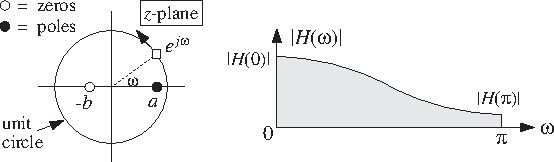
\includegraphics[width = 1\textwidth]{pic/firstOrderFilter.pdf}	
		\end{minipage}
		\textbf{Designparameter des Filters:}
		\begin{itemize}
			\item Steilheit (Stärke) des Filters$\quad\rightarrow\quad$Verhältnis von AC- zu DC-Gain\\[0.2cm]
			\fcolorbox{CadetRed}{white}{$\dfrac{H(\pi)}{H(0)} =\dfrac{(1-b)\,(1-a)}{(1+b)\,(1+a)}\quad\Rightarrow\quad \dfrac{H(\pi)}{H(0)}\begin{cases}< 1 & \text{Tiefpassfilter}\\ >1  &\text{Hochpassfilter}\end{cases}$}
			\item Maximale Zeitkonstante (Einschwingzeit) von $N$ Samples\\[0.2cm]
			\fcolorbox{CadetRed}{white}{$n_{\text{eff}} = \dfrac{\ln(\epsilon)}{\ln(|a|)} \leq N$}
			\item Verstärkungsfaktor $G$ wird oft so gewählt, dass bei einem Tiefpassfilter $|H(0)|=1$ ist und bei einem Hochpassfilter $|H(\pi)|=1$ ist.
		\end{itemize}$ $\\[-1cm]

	\subsection{Resonator}
		Mittels eines konjugiert komplexen Polpaares nahe am Einheitskreis kann ein Resonator gebaut werden. Dabei gelten folgende grundlegenden Zusammenhänge:\\[0.2cm]
		\fcolorbox{CadetRed}{white}{Schmalere Bandbreite$\quad\Leftrightarrow\quad$ Pole näher am Einheitskreis$\quad\Leftrightarrow\quad$ Längere Einschwingzeit des Filters }\\[0.3cm]
		\textbf{Allgemeine Form:}$\qquad$\\[0.2cm]
		\fcolorbox{CadetRed}{white}{$H(z) = \dfrac{G}{(1-R\,\e^{j\omega_0}\,z^{-1})\,(1-R\,\e^{-j\omega_0}\,z^{-1})} = \dfrac{G}{(1 + a_1\,z^{-1}+a_2\,z^{-2}})$}$\qquad$mit $\;\; p = R\,\e^{j\omega_0}$ und $|R|\leq 1$\\[0.2cm]
		\fcolorbox{black}{white}{$a_1 = -2R\cos(\omega_0)\qquad a_2 = R^2$}$\qquad$
		\fcolorbox{black}{white}{$|H(\omega_0)| = 1\quad\Rightarrow\quad G = (1-R)\,\sqrt{1-2R\cos(2\omega_0)+R^2}$}\\
		\begin{minipage}{0.47\textwidth}
			\textbf{Bandbreite als Designparameter:}\\[0.2cm]
			Die $3\db$ Bandbreite ist die Breite auf der halben maximalen Höhe des quadrierten Frequenzganges.\\[0.2cm]
			\text{\textcolor{white}{$\Rightarrow\quad$}}\fcolorbox{CadetRed}{white}{$\Delta\omega = \omega_2-\omega_1$}$\qquad$
			\fcolorbox{CadetRed}{white}{$|H(\omega_{1,2})|^2 = \dfrac{|H(\omega_0)|^2}{2}$}\\[0.2cm]$\quad\Rightarrow\quad$\fcolorbox{CadetRed}{white}{$10\log\left(\dfrac{|H(\omega_{1,2})|^2}{|H(\omega_0)|^2}\right) = 10\log\left(\dfrac{1}{2}\right)=-3\db$}
		\end{minipage}\begin{minipage}{0.03\textwidth}$ $\end{minipage}
		\begin{minipage}{0.55\textwidth}
			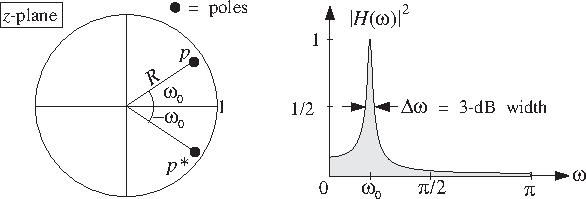
\includegraphics[width = 0.9\textwidth]{pic/resonator.pdf}\\[0.2cm]
			Ist der Pol nahe am Einheitskreis gilt:$\quad$
			\fcolorbox{CadetRed}{white}{$\Delta\omega\approx 2(1-R)$}
		\end{minipage}\\[0.2cm]
		
	\subsection{Notch- und Comb-Filter}
		\begin{minipage}{0.47\textwidth}
			Durch das ''Hintereinanderlegen'' von Polen $(p = R\,\e^{j\omega_0})$ und Nullstellen $(z = r\,\e^{j\omega_0})$ können gezielt bestimmte Frequenzen verstärkt bzw. unterdrückt werden.\\[-0.3cm]
			\begin{itemize}
			\item Pol näher am Einheitskreis ($R>r$)\\
			\text{$\;\Rightarrow\quad$} Verstärkung dieser Frequenz (Comb)\\[-0.3cm]
			\item Nullstelle näher am Einheitskreis ($R<r$)\\
			\text{$\;\Rightarrow\quad$} Unterdrückung dieser Frequenz (Notch)\\[-0.3cm]
			\end{itemize}
		\end{minipage}\begin{minipage}{0.03\textwidth}$ $\end{minipage}
		\begin{minipage}{0.5\textwidth}
			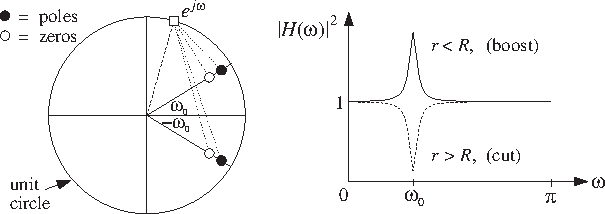
\includegraphics[width = 1\textwidth]{pic/notch.pdf}	
		\end{minipage}\\[0.2cm]
		\textbf{Allgemeine Form:}$\qquad$
		\fcolorbox{CadetRed}{white}{$H(z)= \dfrac{N(z)}{D(z)} = \dfrac{\myprod{i=1}{N}{(1-r\,\e^{j\omega_i}\,z^{-1})}}{\myprod{i=1}{N}{(1-R\,\e^{j\omega_i}\,z^{-1})}}$}$\qquad\quad\begin{array}{l}R<r\quad \rightarrow\quad\text{Notchfilter}\\R>r\quad \rightarrow\quad\text{Combfilter}\\[0.2cm]
		|R|<1\;\;\cap\;\;|r|\leq1\end{array}$\\[0.2cm]

	\subsection{Inverse Filterung}
		\begin{minipage}{0.47\textwidth}
			Oft ist gefordert, eine bestimmte Filterung rückgängig zu machen (z.B. Kanalausgleichung). Dazu kann grundsätzlich die Inverse Filterfunktion verwendet werden.\\[0.2cm]
			\textbf{Inversefilter:}$\qquad$\fcolorbox{CadetRed}{white}{$H_\text{inv}(z) = \dfrac{1}{H(z)}$}
		\end{minipage}\begin{minipage}{0.03\textwidth}$ $\end{minipage}
		\begin{minipage}{0.5\textwidth}
			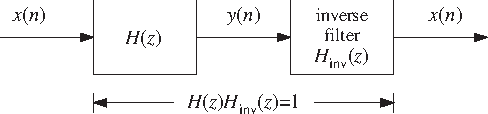
\includegraphics[width = 1\textwidth]{pic/invFiltering.pdf}	
		\end{minipage}\\
		
		Die Inversefilterung hat jedoch zwei bedeutende Probleme:\\[-0.6cm]
		\begin{itemize}
		 \item Das Rauschen wird auch inverse gefiltert.\\[-0.7cm]
		 \item Das Inversefilter muss stabil sein.
		\end{itemize}
		\begin{description}
		 \item [Rauschen:] $ $\newline Wird das verrauschte Signal inverse gefiltert, so wird das Rauschen in den Frequenzbereichen stark verstärkt, in denen das ursprüngliche Filter stark dämpfte $\quad\rightarrow\quad$ Verschlechterung der SNR!\\[0.2cm]
		 \fcolorbox{CadetRed}{white}{$Y(z) = H(z)\cdot X(z) + N(z)\qquad\Rightarrow\quad \hat X(z) = H_\text{inv}(z)\cdot Y(z) = X(z) + \dfrac{N(z)}{H(z)}$}
		 \item [Stabilität des Inversefilters:] $ $\newline
			Ist das ursprüngliche, kausale Filter $H(z)$ stabil (alle Pole innerhalb des Einheitskreises) so heisst dies nicht das das inverse Filter $H_\text{inv}(z)$ auch stabil ist. Durch die Invertierung werden alle Pole zu Nullstellen und alle Nullstellen zu Polen. Dies bedeutet, das Nullstellen, die vorher ausserhalb des Einheiskreises lagen zu Polen werden und das Filter im kausalen Fall dadruch instabil wird. Die Lösung dafür lautet, dass in diesem Fall die akausale Impulsantwort des Inversfilters genommen wird, diese um D Samples verzögert und wenn sie genügend abgeklungen ist (nach D Samples) einfach abgeschnitten wird. Mit dieser Lösung ist das Filter jedoch nur noch eine Approximation des eigentlichen Inversefilters.
		\end{description}